\documentclass[CS4204-Notes.tex]{subfiles}
\begin{document}

\section{Parallel patterns}
A \textbf{pattern} is a common way of introducing parallelism which helps with the program design and helps to guide the implementation. Often a pattern may have several different implementations, for example a \textit{map} can be implemented as a \textit{task farm}. Different implementations may then have different performance characteristics. There are primarily two forms of underlying parallelism: \textbf{data parallelism} and \textbf{task parallelism}.
\begin{figure}[H]
\centering
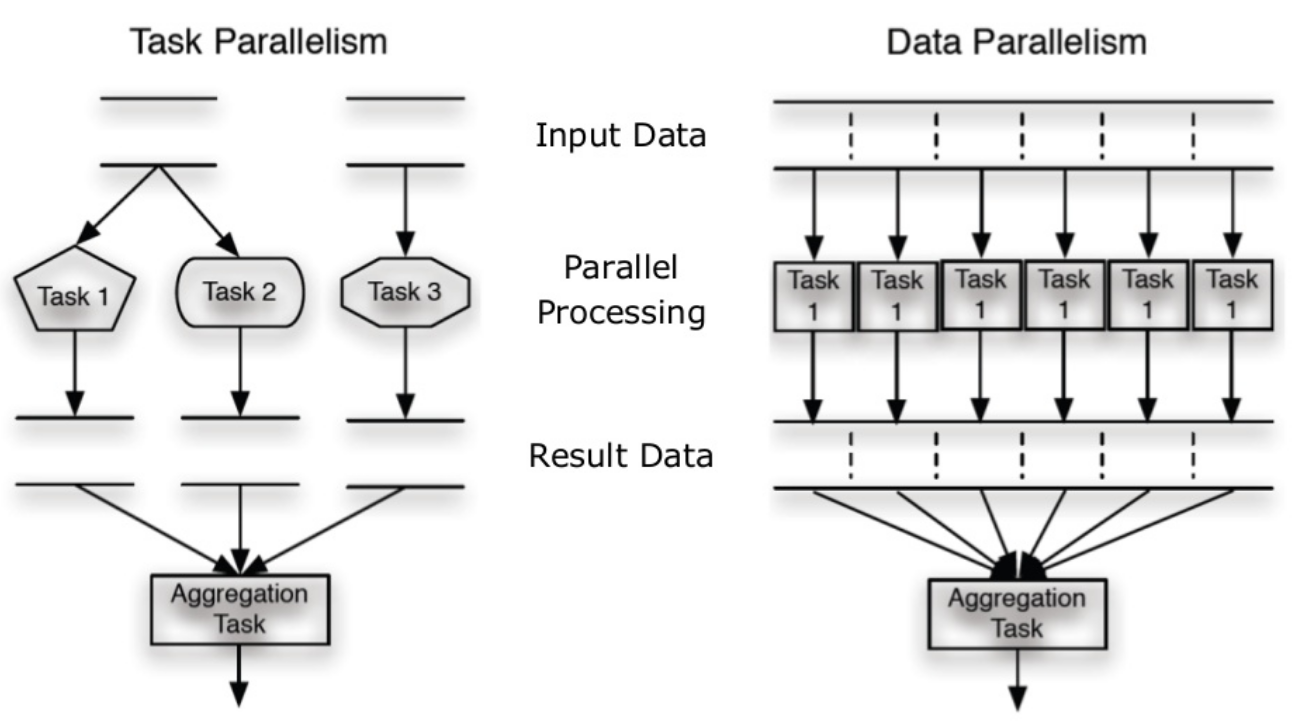
\includegraphics[width=0.7\textwidth, keepaspectratio]{imgs/task-data-parallelism.png}
\caption{Difference between task and data parallelism.}
\end{figure}

\subsection{Data parallelism}
Data parallelism comes from parallelism that is primarily extracted from the structure of the data that operations are applied to. Operations are applied \textit{independently} to several data items, for example the same operation to all elements of a list or array. Data parallelism is generally more regular (that is to say all parallel tasks have similar sizes and functionality) and involves less complex programming structures. Typically data-parallelism may produce large amounts of very fine-grained parallelism which is a good fit for massively parallel architectures like GPUs or SIMD vector architectures. 
\n
Examples of data parallel patterns include:
\begin{itemize}
\item Parallel maps
\item Parallel scans
\item Map-reduce
\end{itemize}

\subsubsection{Parallel maps}
Parallel maps are one of the simplest forms of data parallelism and is also one of the most useful. Sequential maps are very commonly used in sequential Haskell to apply a function to every element in a list. Parallelising this simply involves applying the function in parallel to every element, creating extra threads to evaluate parts of the list. 
\begin{figure}[H]
\centering
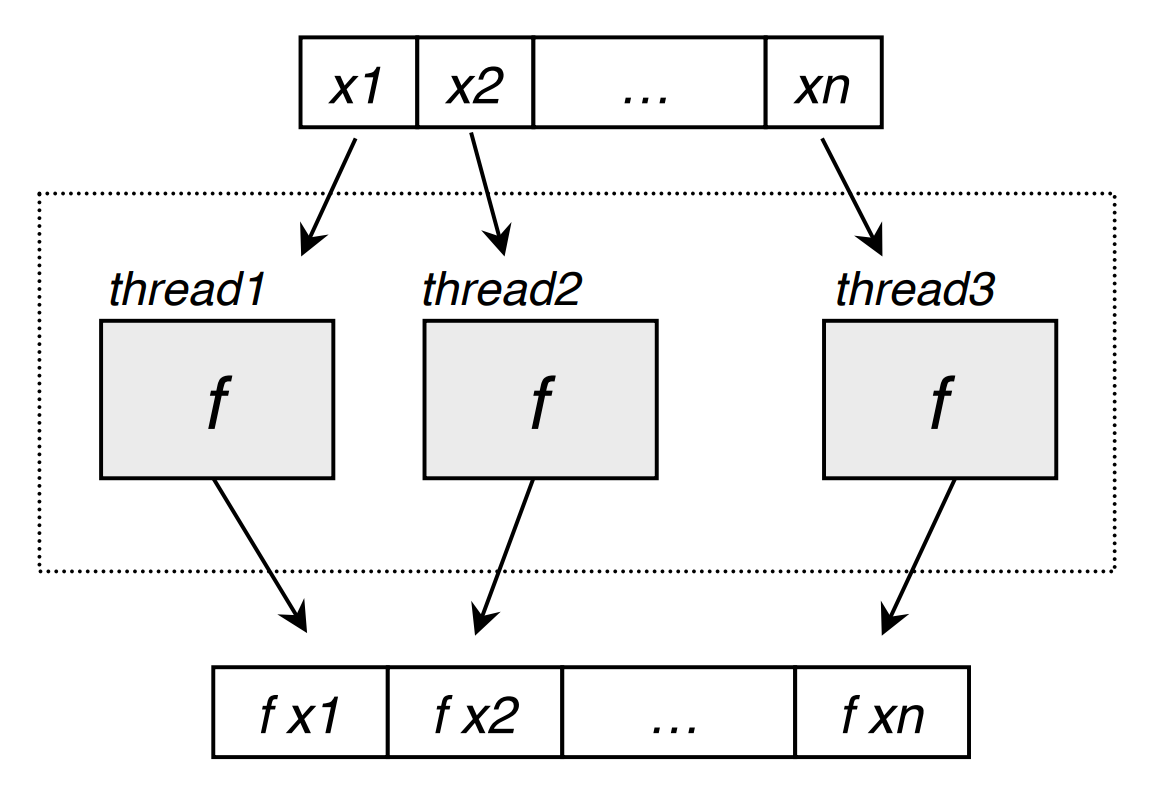
\includegraphics[width=0.5\textwidth, keepaspectratio]{imgs/parallel-map.png}
\caption{Parallel maps map a function across each element in parallel.}
\end{figure}
\noindent

\begin{lstlisting}[caption={Parallel map implementation}]
parmap :: (a -> b) -> [a] -> [b]
parmap f [] = []
parmap f (x:xs) = let fx = f x in
					fx <@\textcolor{red}{\textquoteback par\textquoteback}@> (fx : map f xs)
\end{lstlisting}
\texttt{parmap} can be used anywhere where standard sequential \texttt{map} is used. Although this can be done by simply replace all instances of \texttt{map} with \texttt{parmap}, it may not lead to efficient parallelism. There are a few caveats that need to be taken into account to achieve good parallel performance:
\begin{itemize}
\item All elements of the data structure must already have been evaluated before the \texttt{parmap} is applied
\item There must be no dependencies between the results of the parallel map
\end{itemize}

\subsubsection{Parallel zipWith}
A \texttt{zipWith} is a kind of map that works over two input lists. It maps a function across a pair of elements rather than single elements from one list. The operation \textit{op} is allied in parallel to each pair of elements \textit{x1},\textit{y1} etc. to give the resulting list. The final result is evaluated using a given strategy. As usual, the function calls are only worth evaluating in parallel is the operation \textit{op} is expensive. 
\begin{figure}[H]
\centering
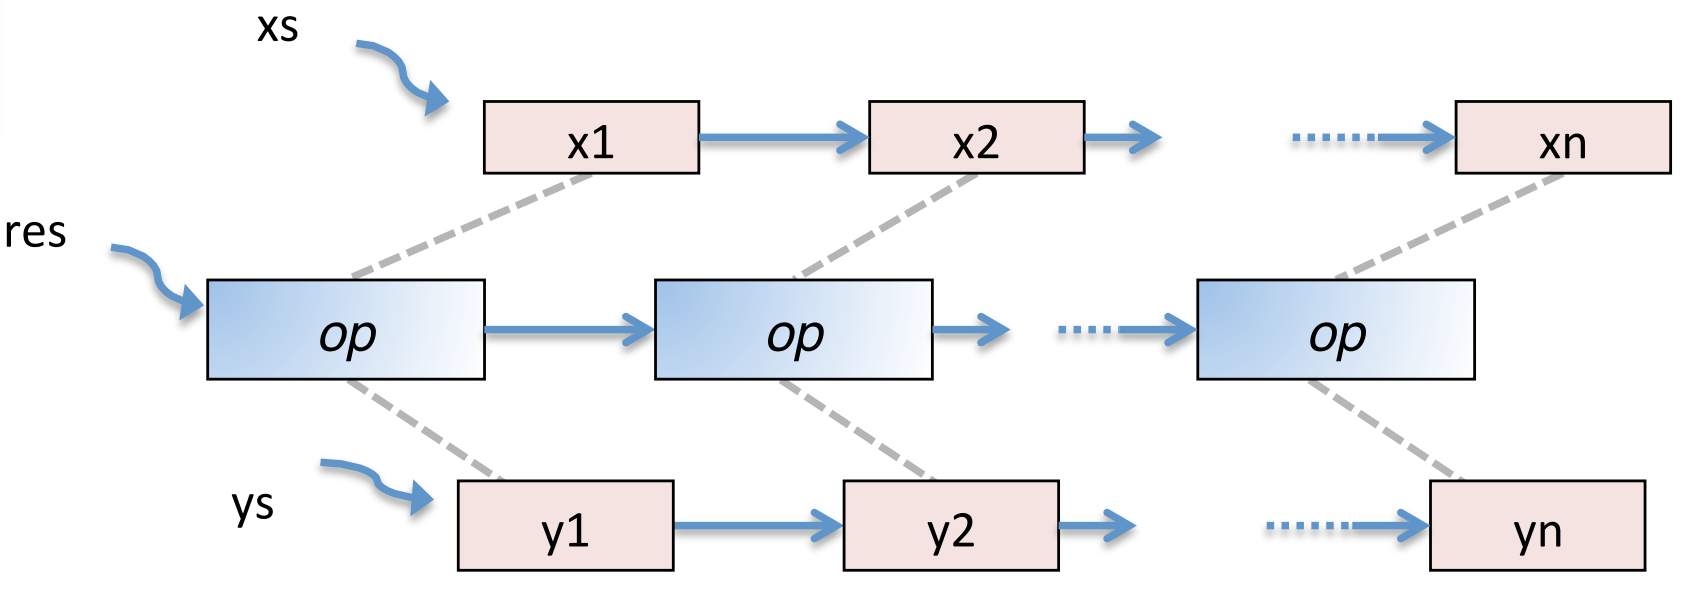
\includegraphics[width=0.9\textwidth, keepaspectratio]{imgs/parallel-zipwith.png}
\caption{Parallel \texttt{zipWith} over two input lists \texttt{xs} and \texttt{ys}}
\end{figure}

\subsubsection{Parallel fold (reduce)}
A fold is a more complex pattern that applies an operator \textit{between} each pair of elements in a list. They can be easily parallelised, however care must be taken over the properties of the operator being used. 
\begin{lstlisting}[caption={Type signature of a parallel fold.}]
parFold :: (a -> a -> a) -> a -> [a] -> a
parFold f z l = ...

-- Examples of fold uses
sum = parFold (+) 0
product = parFold (*) 1
\end{lstlisting}

\begin{figure}[H]
\centering
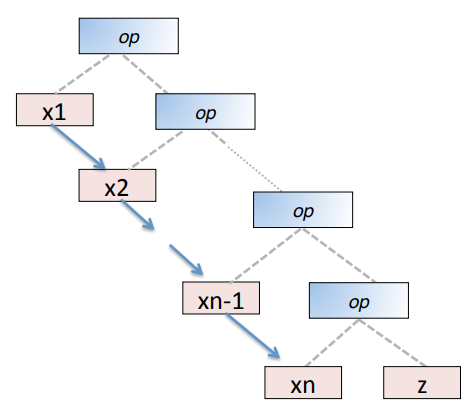
\includegraphics[width=0.5\textwidth, keepaspectratio]{imgs/sequential-fold.png}
\caption{Sequential right fold.}
\end{figure}

\begin{figure}[H]
\centering
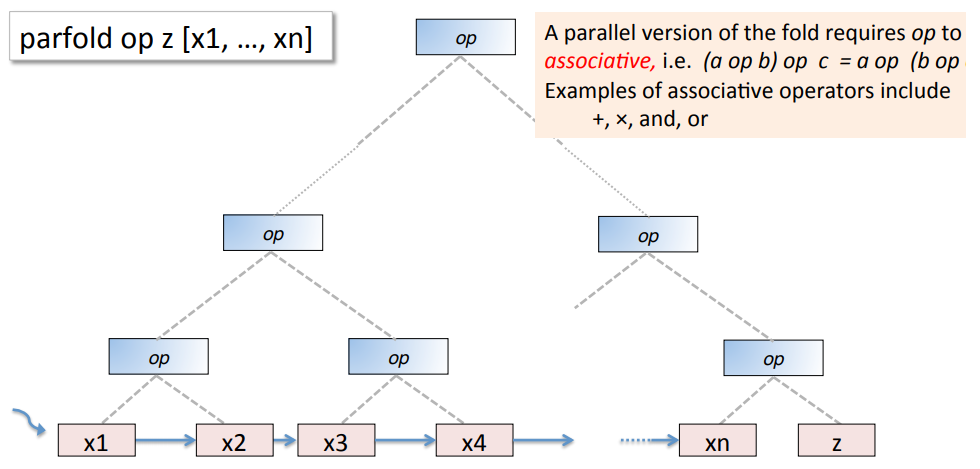
\includegraphics[width=0.9\textwidth, keepaspectratio]{imgs/parallel-fold.png}
\caption{Parallel fold.}
\end{figure}
\noindent
The parallel version of fold requires \textbf{associative} operators because the order of applying the operators cannot matter. This allows the internal computations of the fold to be reordered to give better parallel behaviour. Each operation can be executed by a separate thread and the results combined independently in a tree-like manner. This could not have been done with an associate operator, as the elements of the list cannot be reordered and keep the same result. 

\subsubsection{Bulk Synchronous Parallelism (BSP)}
Bulk synchronous parallelism is a more complicated and sophisticated data-parallel pattern. BSP computations proceeds in a series of \textbf{supersteps} where all threads perform the same computation on different data on each superstep, similar to a parallel map. The difference is that after each superstep, all threads synchronise and exchange some or all data with other threads as needed. The threads are synchronised by barrier, meaning all threads wait until data exchange is completed for all other threads before starting the next superstep. This is potentially very expensive when all other threads are blocked waiting for one or two threads to finish but guarantees that all threads have produced and exchanged information which means no deadlock or livelock. 
\begin{figure}[H]
\centering
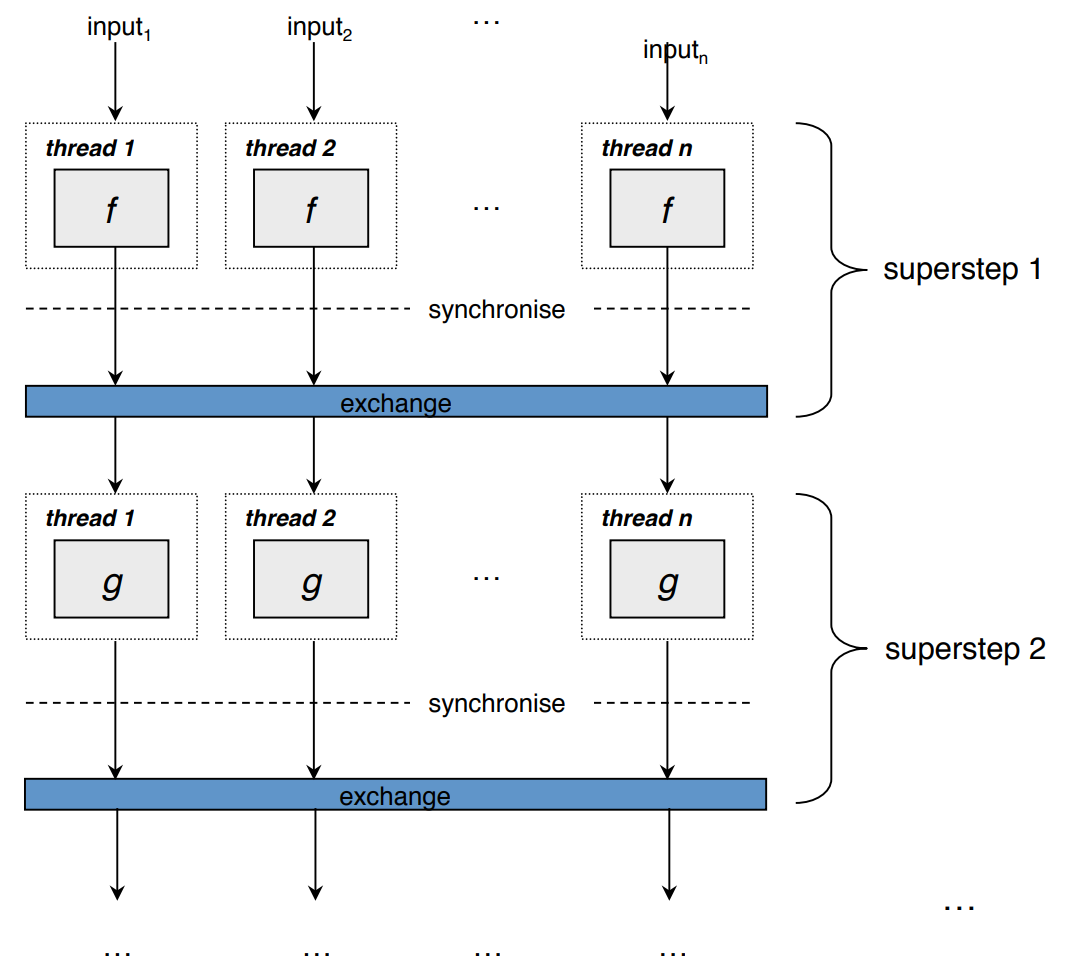
\includegraphics[width=0.6\textwidth, keepaspectratio]{imgs/bsp.png}
\caption{The bulk synchronous parallelism process.}
\end{figure}
\noindent
During each superstep, each thread works on its own inputs using \textit{private local data} and \textit{shared global data}. This global and local data is exchanged between each superstep. The global data from all threads is combined to give a new list of global data, which is then passed as a single value to all of the threads that are evaluating the next worker task. Each thread has its own local state which may be altered as a result of the computation at each superstep. Threads also have access to the global state. During the exchange, each thread produces new local and global state. The global state can only be changed during the exchange. 
\begin{figure}[H]
\centering
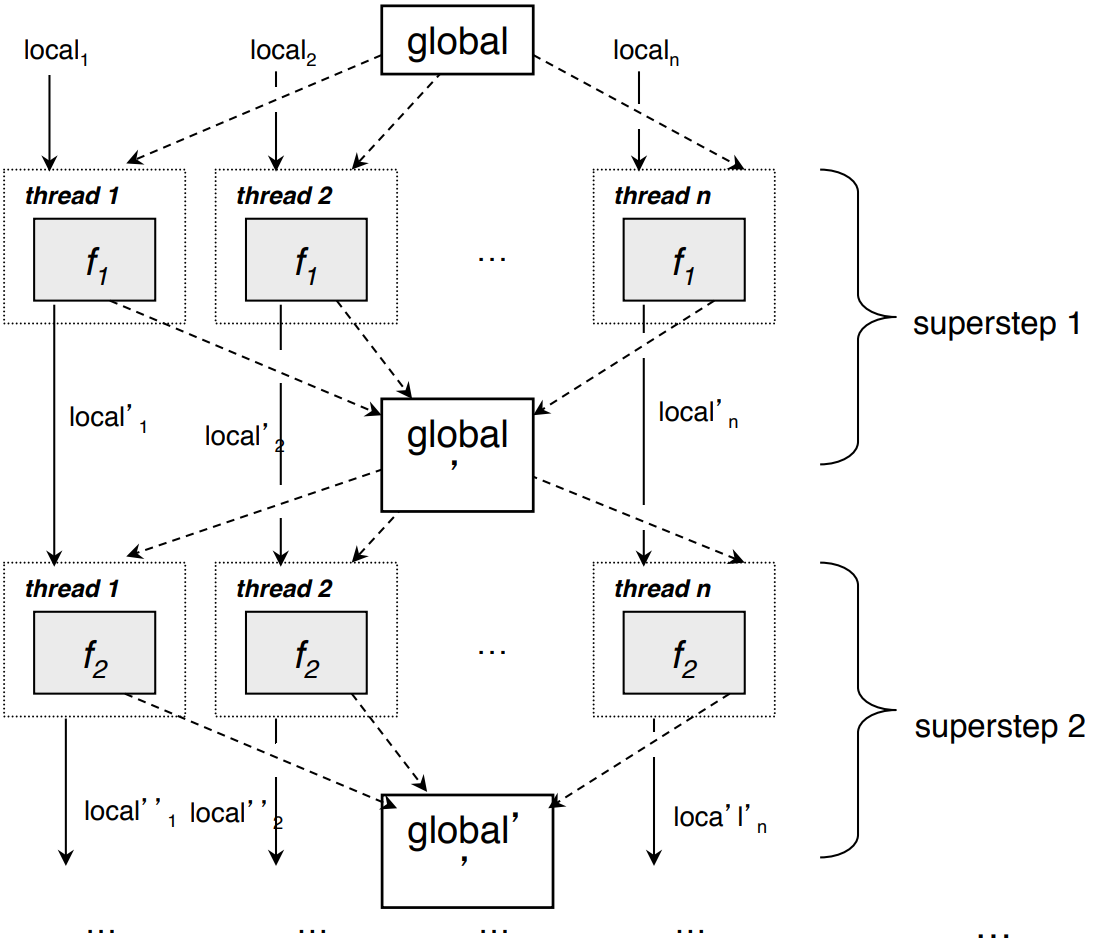
\includegraphics[width=0.6\textwidth, keepaspectratio]{imgs/bsp-exchange.png}
\caption{BSP local and global data exchange process.}
\end{figure}
\noindent
BSP works well when each computation in every superstep has a similar size. The weakness is that in the synchronisation phase, if an operation takes different amounts of time for different inputs, individual threads may be blocked for significant periods of time waiting for other threads to complete. 
\n
The BSP pattern also provides a simple model of parallel execution cost. Since the global synchronisation waits on all threads, the amount of time taken to execute a superstep is always the same for all threads. Further, it follows that the exchange step has the same fixed constant size. This gives the following equation for the time required to execute a complete sequence of $m$ BSP supersteps
\begin{equation}
\sum_{i=1}^{m}f_{i} + c_{ex} \times (m - 1)
\end{equation}
where 
\begin{itemize}
\item $f_{i}$ is the maximum cost of the operation at step $i$
\item $c_{ex}$ is the cost of exchange/synchronisation
\item $m$ is the number of supersteps
\end{itemize}
This calculation assumes that there are enough processors available to execute all of the threads that are created to execute the pattern. 
\subsubsection{Parallel map-reduce}
Map-reduce is a common pattern that has been applied to commercial, large, distributed server farms for dealing with big data. It uses a combination of \textit{map} to map a function across the data and a \textit{reduce} to reduce the results to simpler values. It works by splitting the input into a large number of similarly sized tasks that can be processed independently using the \textit{map} operation. Then each intermediate group of data can be processed with the \textit{reduce} function. 
\begin{figure}[H]
\centering
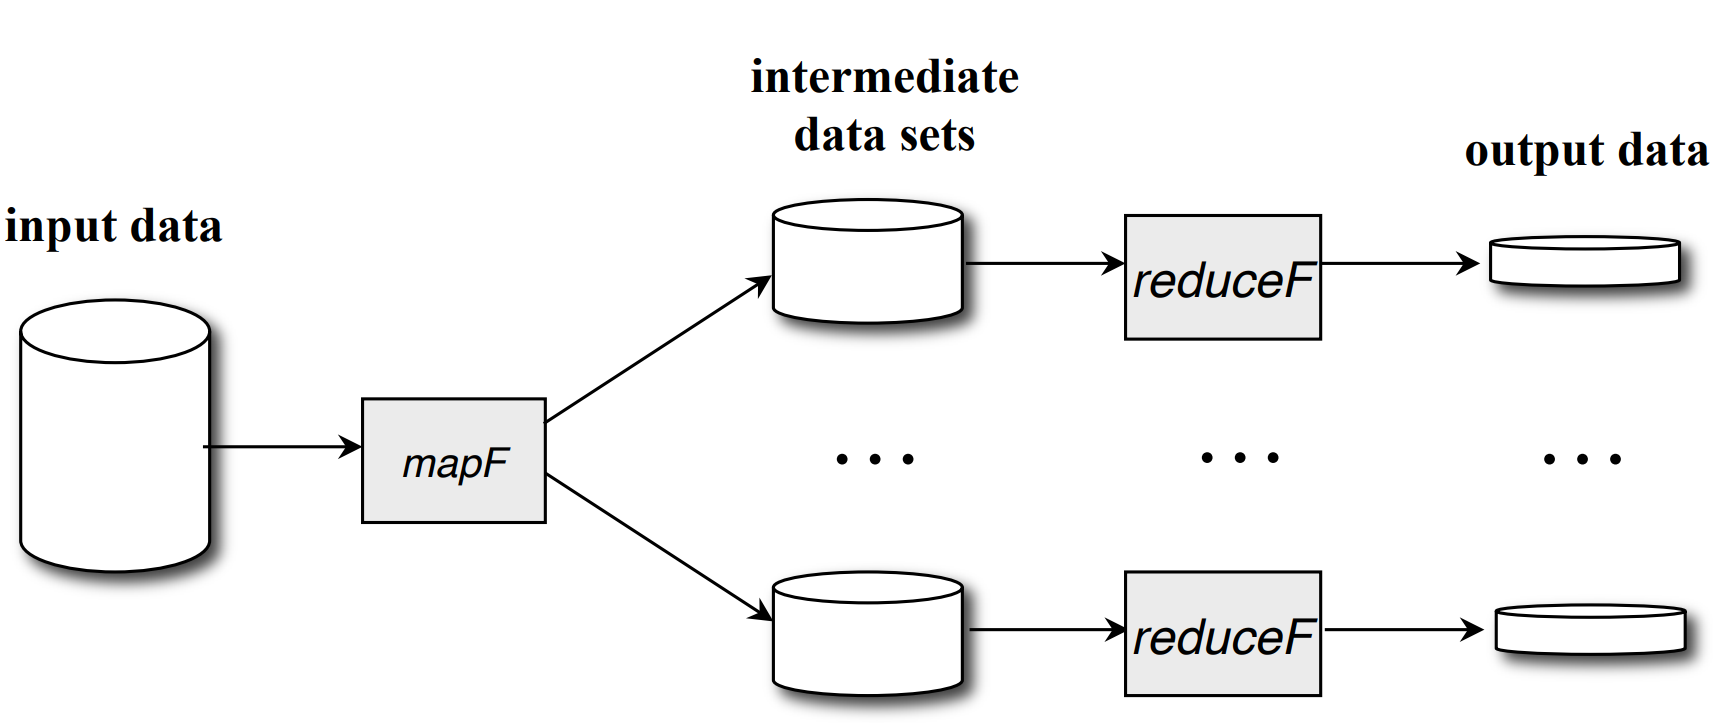
\includegraphics[width=0.9\textwidth, keepaspectratio]{imgs/map-reduce-simple.png}
\caption{Map-reduce with parallel reduction step.}
\end{figure}
\noindent
Quite clearly the reduce operations can be run in parallel with data parallelism, using a parallel map to map the reduce function to the data. However, it is also possible to increase the parallelism by running the map operations in parallel by splitting the data and them mapping each map in parallel. If the reduction operation is associative, each set of intermediate results may then be reduced independently: a local reduce function is applied to each intermediate set of results and an overall reduce function applied at the end of get the final result. 
\begin{figure}[H]
\centering
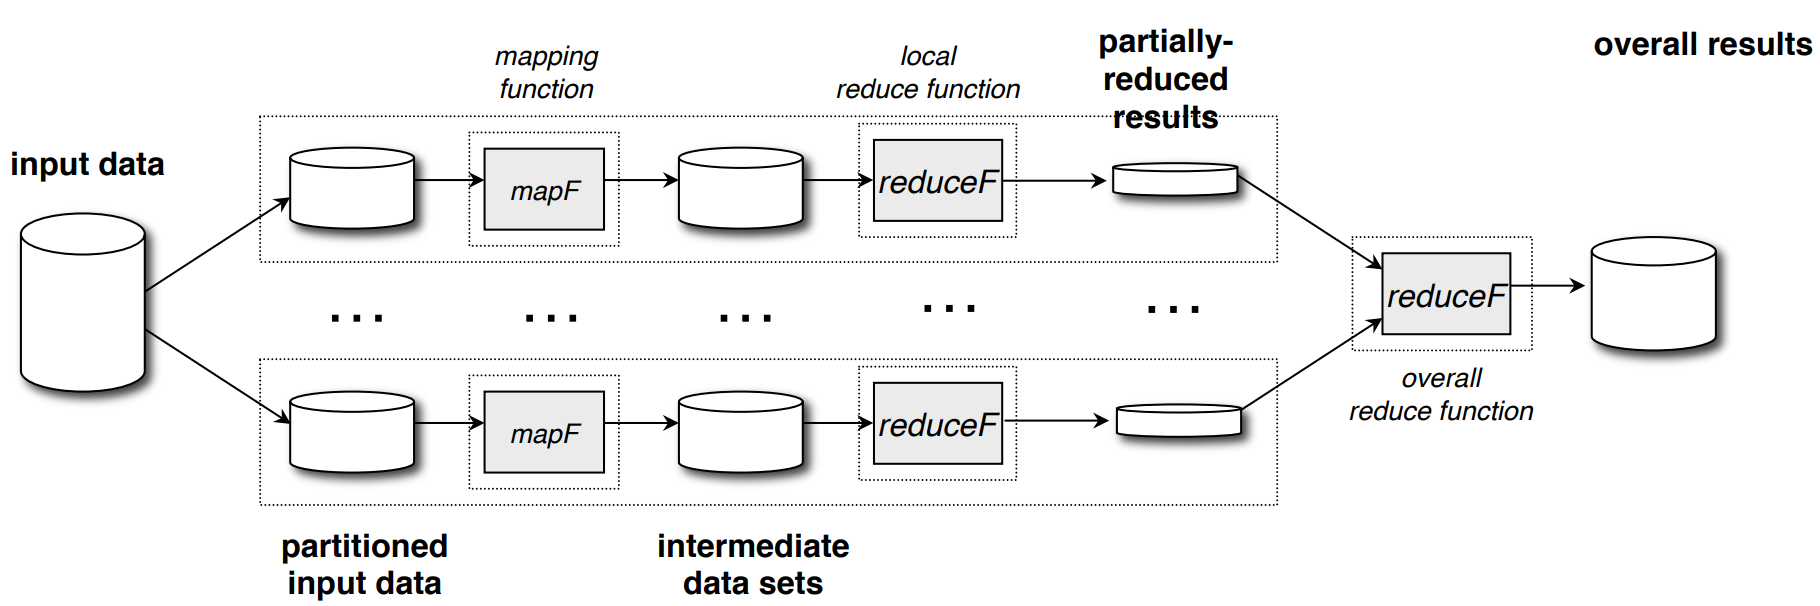
\includegraphics[width=1\textwidth, keepaspectratio]{imgs/map-reduce-more.png}
\caption{Map-reduce with parallel mapping step.}
\end{figure}

\subsubsection{Parallel scan}

\subsection{Task parallelism}
In contrast to data parallelism, task parallelism comes from the control flow in a program. This is more flexibly than data-parallelism but often exposes less parallelism and is harder to conceptualise. Further, task-parallelism has a less regular size and structure, as each part of the control flow can have different functionality, making it difficult to manage at runtime. 
\n
Examples of task parallel patterns include:
\begin{itemize}
\item Piplines
\item Divide and conquer
\item Task farm
\end{itemize}
Task parallelism aims to deal with issues in data parallelism, mostly to do with irregular thread granularities. For example in BSP, if the thread granularities are not balanced, some cores may remain idle, wasting possible computation time. This is where task parallelism comes in. It is parallelism that does not come purely from the structure of the data, where computations are not the same for each item and where there are irregular granularities.
\n
In general, task parallelism is much harder to handle compared to data parallelism for the following reasons:
\begin{itemize}
\item Less regular
\item Harder to map to the available resources
\item Can give much less parallelism
\item Can be harder to identify the patterns
\item May need specialist support to implement
\end{itemize}
However, because many problems cannot be solved by data parallelism, task parallelism must be used in these cases.

\subsubsection{Producer-consumer}
Producer-consumer is one of the simplest patterns of task parallelism. One thread produces values which another thread consumes. If the producer produces only one simple value, then there is very limited scope for parallelism, however if the producer produces a lazy list or incrementally constructed structure, then each element can be consumed as soon as it is produced.
\begin{figure}[H]
  \centering
  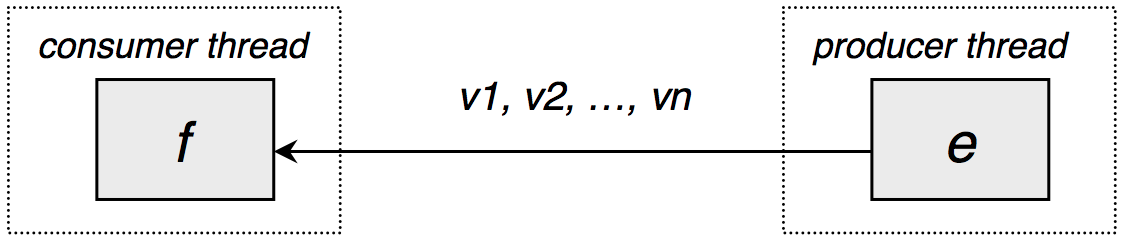
\includegraphics[width=0.75\textwidth, keepaspectratio]{imgs/producer-consumer.png}
  \caption{Producer-consumer parallelism. If the original sequential operation is \texttt{f \$ e}, then the parallel version is \texttt{f \$|| rdeepseq e}.}
\end{figure}
\noindent
The producer-consumer pattern can be easily implemented using \texttt{\textquoteback par\textquoteback}
\n
\begin{minipage}{0.45\textwidth}
\begin{lstlisting}[caption={Sequential producer-consumer}]
f $ e = f e
\end{lstlisting}
\end{minipage}
\hspace*{\fill}
\begin{minipage}{0.45\textwidth}
\begin{lstlisting}[caption={Parallel producer-consumer}]
f $| e = e `par` f e
\end{lstlisting}
\end{minipage}
This works because by exploting Haskell's lazy evaluation to pass the result from the producer to the consumer as it is produced.

\subsubsection{Parallel pipelines}
Pipelines are an extension of the producer-consumer parallel pattern. In essence the pipeline is a combinations of a series of producer-consumer operations over a stream of inputs.
\begin{figure}[H]
  \centering
  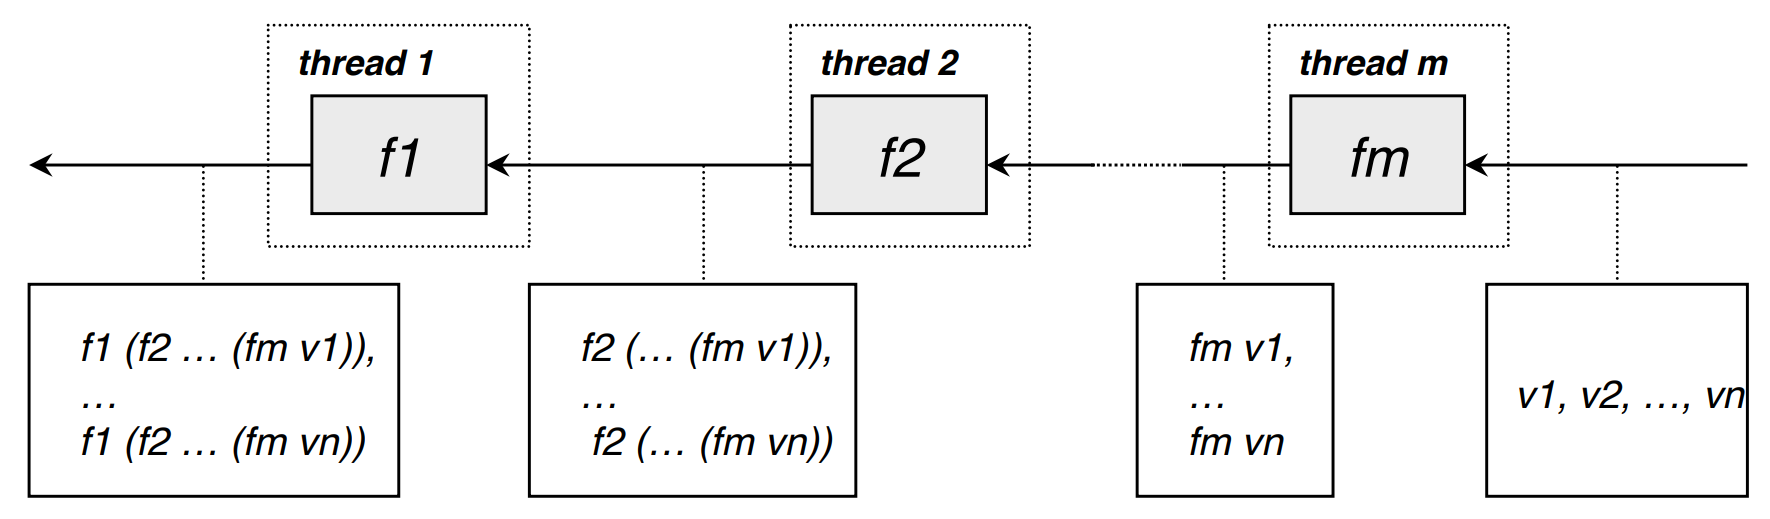
\includegraphics[width=0.9\textwidth, keepaspectratio]{imgs/parallel-pipeline.png}
  \caption{Parallel pipeline where each thread executes a different function $f$.}
\end{figure}
\noindent
In the sequential version, a pipeline simply applies on function after another to the input \texttt{x}, giving \texttt{pipeline3 f1 f2 f3 x = f3 \$  f2 \$ f1 \$ x}. The parallel version uses the \texttt{\$||} operator to add a strategy to each stage that is applied to the input argument in parallel with the evaluation function.

\subsubsection{Parallel streams}
Streams are the natural extension of a pipeline where the operations are repeated over multiple values. The stream produces results in the order that the inputs are given, in other words, there is exactly one output produced for each input value. This is done simply by applying a \texttt{map} to each argument function
\begin{lstlisting}[caption={Parallel stream pattern on a three-stage pipeline.}]
parstream3 f1 f2 f3 = parpipeline (map f1) (map f2) (map f3)
\end{lstlisting}
This completely encapsulates the three-stage pipeline as a streaming definition. Of course this can be generalised to an arbitrary number of stages using a list instead of specifying each function seperately. The drawback to this generic method is that each function must have the same type
\begin{lstlisting}[caption={Arbitrarily sized \texttt{parstream} using a list of functions \texttt{fs}.}]
  parpipeline fs z =
    foldr (\f x -> f $|| rdeepseq $ x) z fs

  parstream fs l =
    parpipeline (map map fs) l
\end{lstlisting}

\subsubsection{Divide and conquer}
The divide and conquer pattern is one that commonly occurs in parallel computation and is a pattern that can be easily identified. It works by splitting the data into two or more independent parts so that each part can be worked on in parallel and the results combined at the end to give the final result. Sometimes we wish to divide until the problem is small enough to be trivially solvable, but this depends on the optimal granularity.
\begin{figure}[H]
  \centering
  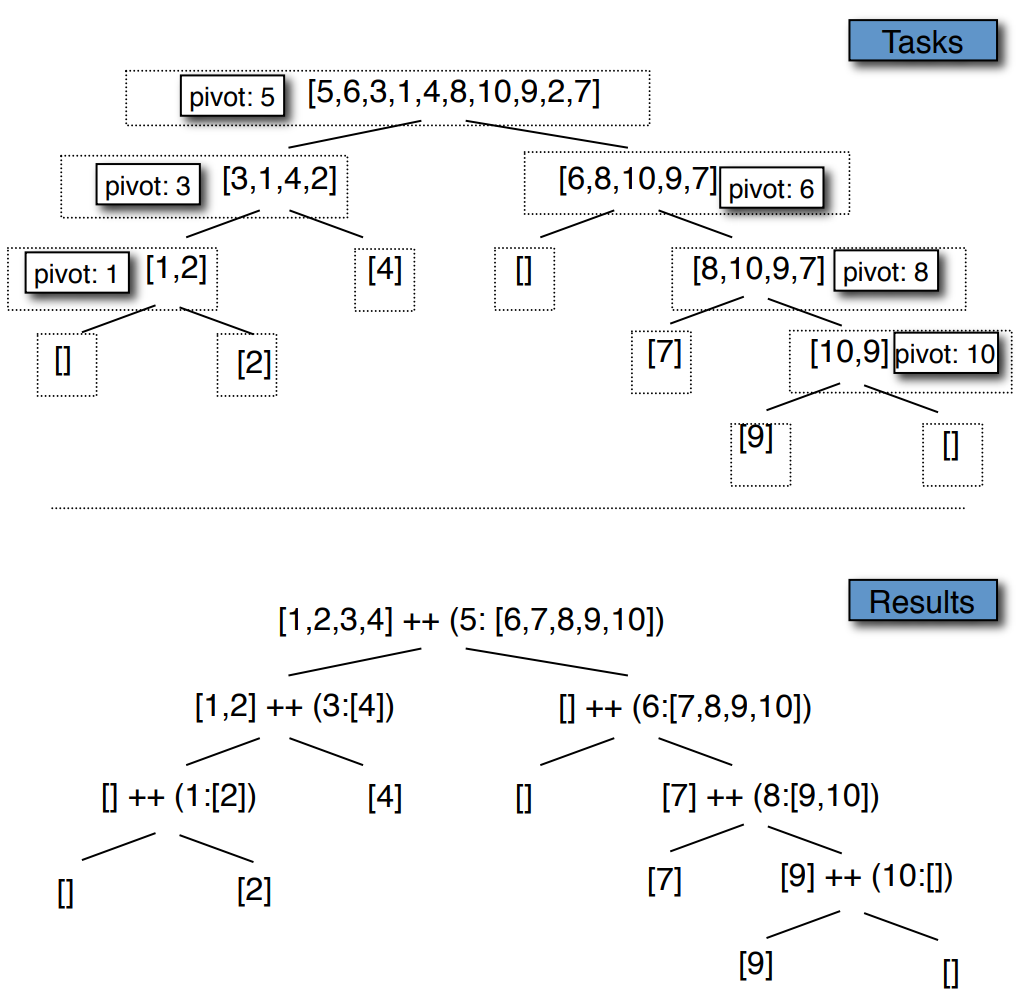
\includegraphics[width=0.65\textwidth, keepaspectratio]{imgs/divide-and-conquer.png}
  \caption{Example of divide and conquer with quicksort, dividing the input until the trivial case.}
\end{figure}
\noindent
The strength of divide and conquer comes from the fact that it is completely recursive to the base case. In other words, each sub-divided task can be further divided with the same divide and conquer approach. The has several benefits:
\begin{enumerate}
\item A large number of tasks can be generated very rapidly
\item Can be quickly spread across a parallel system - this is especially important for distributed memory systems
\item Communication paths are well-defined and hierarchical - again important for distributed memory systems
\item No single processor becomes overloaded with the task of distributing work and combining results as the division can be done recursively on separate processors
\end{enumerate}
The concept of \textbf{thresholding} is important to ensure the right granularity is found. We do not want tasks that are too small or trivial as the overhead of creating threads for these tasks will be greater than the amount of work gained from parallelising the work. The idea is to deliberately create larger tasks either once enough parallelism is created, or when the new tasks created fall below some threshold size. Tasks smaller than the threshold are not further divided and are processed sequentially.
\n
This allows one to control the size of the parallel tasks that are created by varying the \texttt{threshold} value. It should be noted that if the size of the input list is large, the calculation of the length of the list can be expensive. In this case, it may be more effective to track the depth of the tree rather than the length of the input and only parallelise down to a certain depth.
\n
There are three components to the \textbf{general divide and conquer} pattern
\begin{enumerate}
\item The input data is split into two or more parallel tasks
\item When the tasks are small enough, based on some threshold or depth, a sequential worker function is applied to the input
\item The results from the split tasks are combined to give an overall result that is returned to the next higher level in the tree
\end{enumerate}
This gives a general pattern than can be used in a variety of situations.
\begin{lstlisting}[caption={A general divide and conquer pattern}]
  dc :: Strategy b -> (a -> [a]) -> (a -> Bool) -> ([b] -> b) -> (a -> [b]) -> a -> b
  dc strat splitf thresholdf combinef seqworkerf input = combinef results
    where results =
      if thresholdf input then
        seqworkerf input
      else
        parMap strat (dc strat splitf thresholdf combinef seqworkerf) (splitf input)
\end{lstlisting}

\subsubsection{Task farms/workpools}
In a task farm (also called master-slave) system, a number of worker processes are coordinated by a single master process. The master process decides which task should be executed by which worker, then it allocated the task to the chosen worker and receives the result from each work and merges the results into the result stream.
\begin{figure}[H]
  \centering
  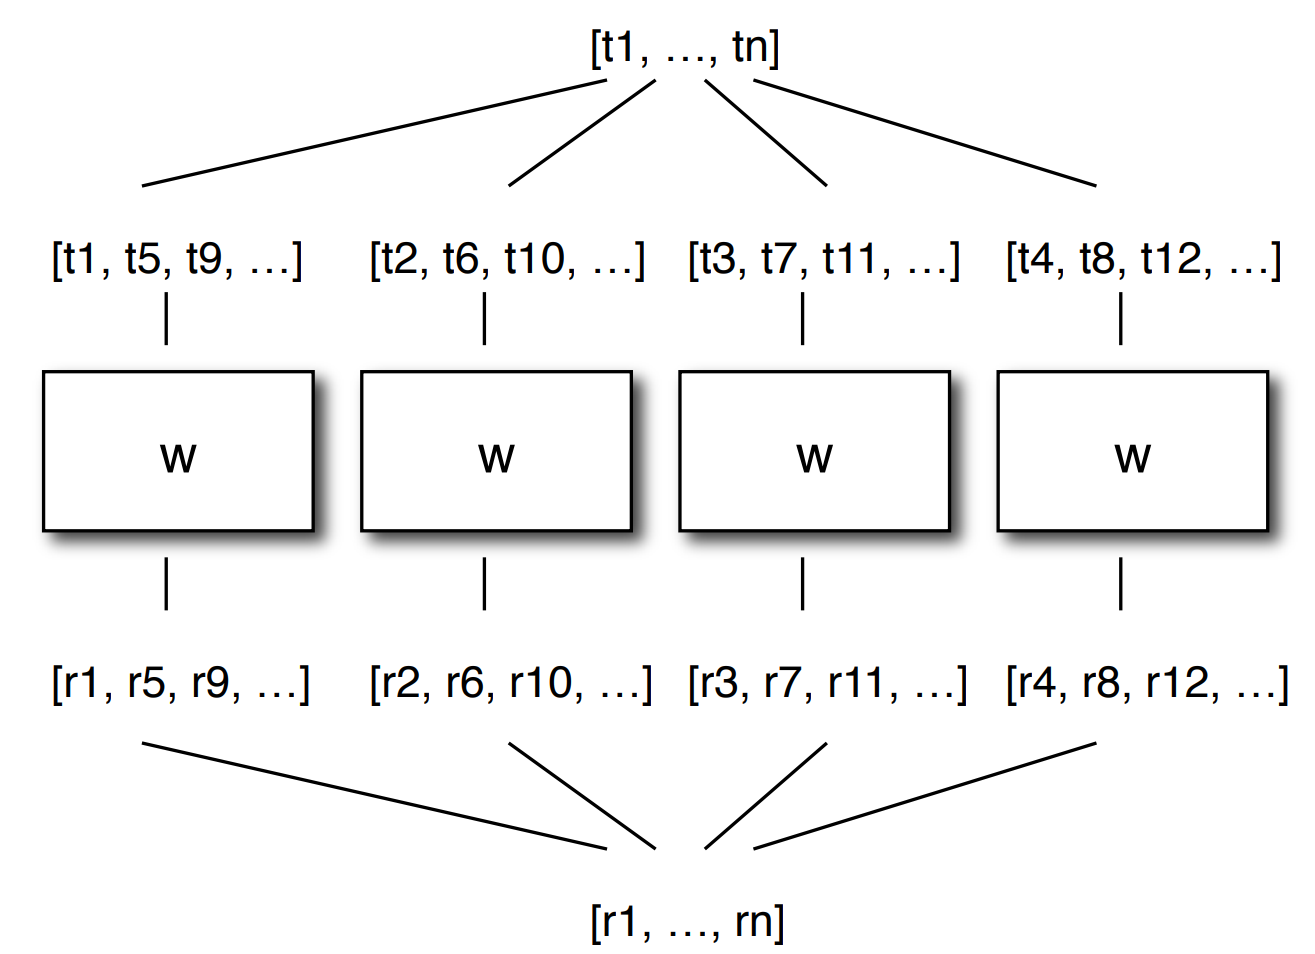
\includegraphics[width=0.45\textwidth, keepaspectratio]{imgs/taskfarm.png}
  \caption{A parallel task farm with 4 workers.}
\end{figure}
\noindent
In general, the tasks are allocated to workers equally. Each coarse grained worker can execute a fine grained task, which saves on thread creation overhead.
\begin{lstlisting}[caption={General parallel task farm implementation.}]
  taskFarm :: Strategy [b] -> (a -> [b]) -> Int -> [a] -> [[b]]
  taskFarm strat f nWorkers tasks = concat results `using` parList strat
    where results = unshuffle nWorkers (map f tasks)

  unshuffle :: Int -> [a] -> [[a]]
  unshuffle n xs = [takeEach n (drop i xs) | i <- [0..n-1]]
      where takeEach :: Int -> [a] -> [a]
        takeEach n [] = []
        takeEach n (x:xs) = x : takeEach n (drop (n-1) xs)
\end{lstlisting}

\subsubsection{Workpools}
A parallel workpool is similar to a task farm except that it tracks which worker has completed a task before assigning it the next task from the list of input tasks. In other works the tasks are dynamically allocated as they are completed. This allows the workpool to deal with collections of tasks, where the tasks may have widely differing sizes.
\begin{figure}[H]
  \centering
  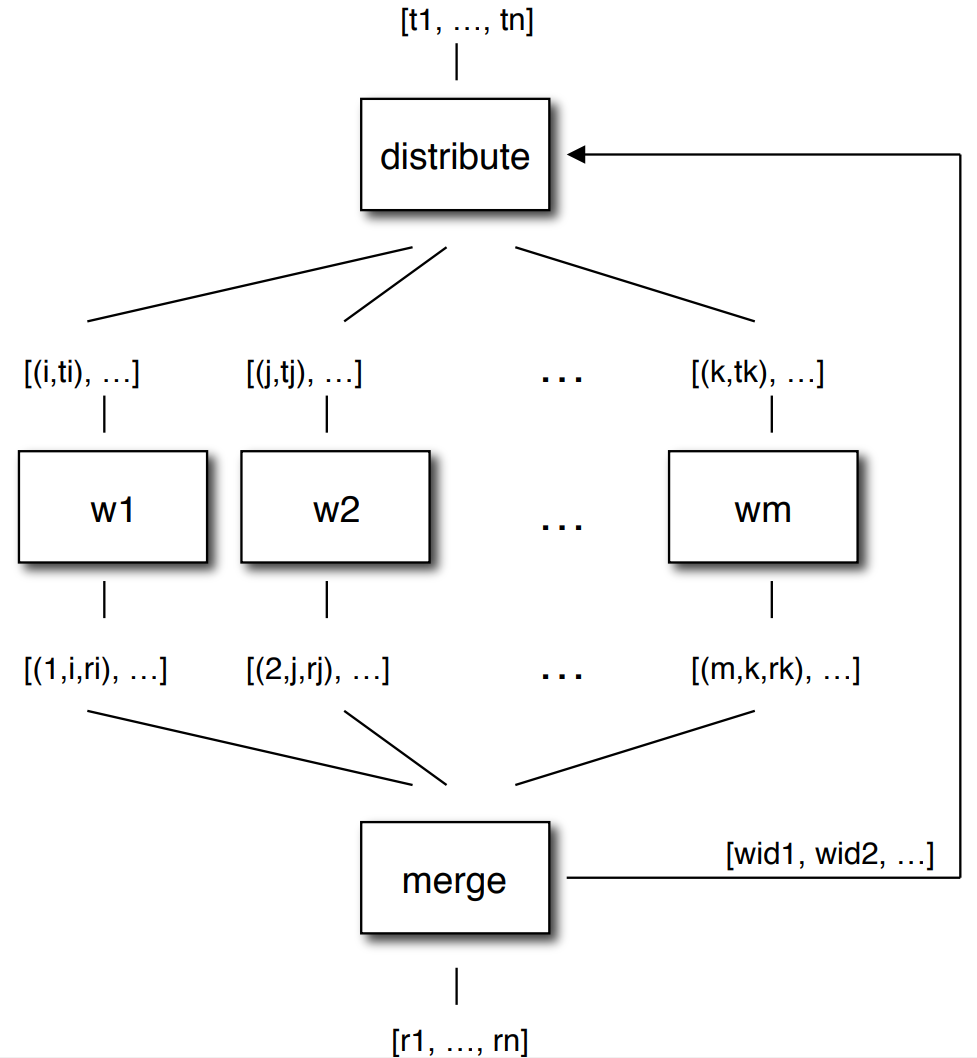
\includegraphics[width=0.45\textwidth, keepaspectratio]{imgs/workpool.png}
  \caption{Parallel workpool, which dynamically allocates tasks to workers as they are completed.}
\end{figure}

\subsubsection{Parallel search}
Parallelism can be used to speed up search in a data structure. In a search problem, we are looking for the existence of some value, so each individual search can be run in parallel. Moreover, any solution is acceptable, so the search an stop when the value is found.
\begin{lstlisting}[caption={Parallel search by applying \texttt{parmap} on the \texttt{find} operation.}]
  parSearch :: (a -> Bool) -> [a] -> Bool
  parSearch find l = any (== True) (parmap find l)

  any p [] = False
  any p (x:xs) = p x || any p xs
\end{lstlisting}

\subsubsection{Branch and bound parallelism}
\begin{figure}[H]
  \centering
  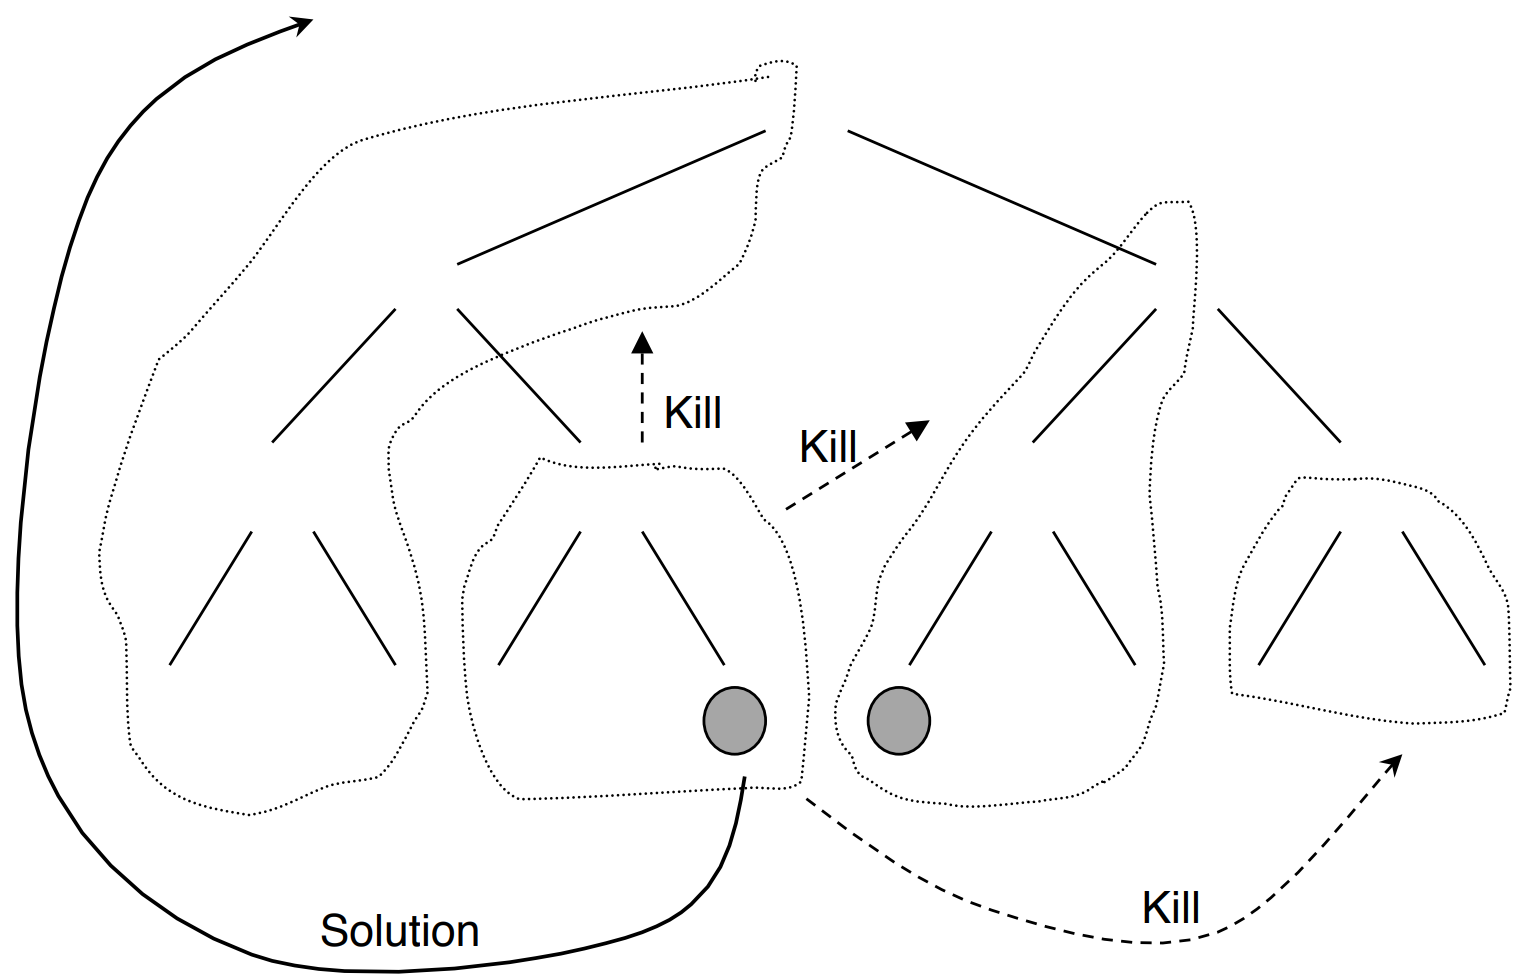
\includegraphics[width=0.75\textwidth, keepaspectratio]{imgs/branch-and-bound.png}
  \caption{In branch and bound, parallel search threads are killed once the solution is found.}
\end{figure}

\end{document}